\chapter{Results and Discussion}
\label{sec:R&D}

In this nearly two year long study, we have managed to investigate a great number of materials with various structures and compositions. We initially began by experimenting with an $Fe_2Si$ unit cell and create these high-entropy silicides by using the special quasi-random structure approach as described above. All though this initial compound is not a semiconductor, we worked under the hope that the extraordinary properties that have been observed in high-entropy alloys through effects such as the cocktail effect, we could locate a specific combinations of elements that in terms would yield a semiconductor with unchanged metal to silicon ratio. Thus creating a highly efficient thermoelectric material based on the other suitable properties of di-iron silicide.  All though this idea is not invalidated, because there are plenty-full of else compositions and permutations to trial, in our narrow search we however did not find such a material. Therefore we opted for a more conservative angle for our study by instead considering well known semiconducting TM silicides such as $\beta - Fe_2Si$, $CrSi_2$ and $MnSi_{1.75}$, see section .. for an introduction to these. However, also for these disilicides we experiences limited success in finding semiconducting materials. In fact, the only case in which we found positive confirmation of a band gap was for a particular composition of $(Cr_{0.25}Fe{0.25}Mn_{0.25}Ni_{0.25})Si_2$, here-in CFMN, in the $\beta FeSi_2$ configuration. This make for an interesting question that we will try to understand and answer in this section, why is exclusively this compound semiconducting?  

We will try to answer this question by first considering the CFMN (fesi2) compound, and investigating the potential properties and correlations between the different elements that make this particular system semiconducting. Factors we will investigate is the overall stability by total energy per atom and formation enthalpy, the magnetic configuration and which elements contribute the magnetism. But in majority, we will look at the band gap and related properties, as this is the main motivation and distinction of the study. When we are done analyzing this system, we will transition into the similar compounds we have worked with in this project, but that turn out metallic. First we will look at compounds within the same crystal structure, but where we substitute the exact composition of $(Cr_{0.25}Fe{0.25}Mn_{0.25}Ni_{0.25})Si_2$ with other 3d elements and distributions slightly away from eqvimolar. Then we present the results of the CFMN composition in different crystal structures mentioned above, ie $Fe_2Si$ where we flip the metal-silicon atom ratio, $CrSi_2$ where the ratio is consistent, but in a different crystal structure, and $MnSi_{1.75}$ where we alter both simultaneously. Finally we will compare and discuss the observed distinctions and give our thoughts on the complete experiment and guideline future research directions in this field.     

\section{One iron, two silicide}
In section .. we briefly discussed various semiconducting TM silicides, such as $\beta-FeSi_2$ in the orthorombic cmce lattice. In our DFT work, we find this structure semiconducting with an indirect band gap close to 0.65 eV with PBE. Additionally we found the compound to be non-magnetic and a total energy per atom equal to 6,8274 eV. Which means that we can calculate the formation enthalpy as $\Delta H = E/at_{FeSi_2} - (E/at_{Fe} + E/at_{Si})$ = 7,0653 eV, with the help of materials project for providing the total energy per atom for iron (-8.4693 eV) and silicon (-5.4234 eV).

The $FeSi_2$ structure consisted of 48 atoms, 16 of which is iron and the remaining 32 sites occupied by silicon atoms. In our project, we filled the 16 iron sites with an even distribution of chromium, iron, manganese and nickel by the principle of the SQS method described in section .. . With this approach, there are many possible supercells one can create, we however limit our-self to 5 distinct supercells per composition, which means that we have 5 structures of the same composition and space group, but the distribution is slightly different. This allow us to both study a composition to great depth, but also to test different compositions and structures, compared to if we instead generated 10 or 15 or more supercells. But its important to be aware of this assumption, as our results may be subject to errors and result that does not match the true random alloy due to a small sample size.

\subsection{CFMN (fesi2)} 

Bellow in table .. we display the most relevant properties to the 5 SQSs of the CFMN (fesi2) system for this study, they are the total energy per atom, final magnetic moment per atom, and the band gap. For simplicity, we denote these SQSs as A, B, C, D and E.   

\begin{table}[H]
\centering
\begin{tabular}{@{}cccc@{}}
\toprule
Structure  & Total energy/atom (eV) & Final magnetic moment/atom (?) & Band gap (eV) \\ \midrule
\textbf{A} & −6,6080                & 0.0833                    & 0.0280        \\
\textbf{B} & −6,6138                & 0.0833                    & 0.0523        \\
\textbf{C} & −6,6063                & 0.0834                    & 0.0344        \\
\textbf{D} & −6,6155                & 0.0833                    & 0             \\
\textbf{E} & −6,6089                & 0.0833                    & 0.0495        \\ \midrule
\textbf{Mean} & -6.6105 & 4.0000 & 0.0328    \\
\textbf{Std} & 0.0039 &  - &  0.0210 \\
\textbf{$\Delta H_{mean}$} & 31,8767 eV \\ \bottomrule
\end{tabular}
\caption{Total energy per atom, final magnetic moment, band gap (GGA) and formation enthalpy of $Cr_4Fe_4Mn_4Ni_4Si_{32}$ SQSs based on $FeSi_2$}
\label{table:fesi2_summary}
\end{table}  

From a first glance, we observe very similar properties between the structures regarding both the total energy and final magnetic moment. \textbf{Something on stability}. Comparing to $FeSi_2$, by replacing purely iron atoms with a number of 3d elements we have made the compound magnetic. We performed self-consistent total energy calculations with ispin=1, ispin=2 and ispin=2, MGMOM=2*NIONS \textbf{What does this mean?}, and found that ispin2 was the most stable magnetic configuration. The consistent magnetic moment between the 5 supercells is excpected seeing as all 5 structures consist of equivalent elements. The magnetism is as attributed solely from 3d electrons and in particular from chromium and manganese, whereas the iron and nickel atoms are diamagnetic. \textbf{Near 0, or negative values in OUTCAR}. 
 
The most interesting property of these SQSs is in fact the band gap. We note a mean band gap of about 0.03 eV, in contrast to 0.65 eV in bulk $FeSi_2$. The gap is seen in 4 out of 5 SQSs, but surprisingly not in the most stable arrangement (D), the largest gap observed is about 0.05 eV from structure B, which is very similar to D in terms of total energy. Moreover the gaps are indirect, the transitions is listed bellow in table .. .     

\begin{table}[H]
\centering
\begin{tabular}{@{}ccc@{}}
\toprule
Structure  & Gap (D/I) & Transition                              \\ \midrule
\textbf{A} & I         & (0.500,0.333,0.500)-(0.500,0.000,0.000)  \\
\textbf{B} & I         & (0.250,0.000,0.250)-(0.000,0.000,0.000)  \\
\textbf{C} & -         & (0.500,0.000,0.500)-(-0.250,0.333,0.500) \\
\textbf{D} & I         & -                                        \\
\textbf{E} & I         & (0.000,0.000,0.000)-(0.250,0.000,0.250)  \\ \bottomrule
\end{tabular}
\caption{Band gap transition of CFMN (fesi2) SQSs with PBE functional}
\end{table}

A very useful method to extract information regarding the band gap of a material is to plot and study the band structure, however this is not as insightful when considering large supercells with large number of energy bands. The solution to this is normally to do a band unfolding, but given the complex structure and implementation of these SQS is VASP we where not able to do band-unfolding or plot the band structure in any way. Another method to study the band gap is to observe the density of states, in figure .. we plot the total density of states. In these plots, the 0 value on the x-axis is set to the Fermi energy, in other word the negative values relate to states in the conduction band and positive values the valence band. 

\begin{figure}[H]
	\centering
	\begin{subfigure}{0.9\textwidth}
		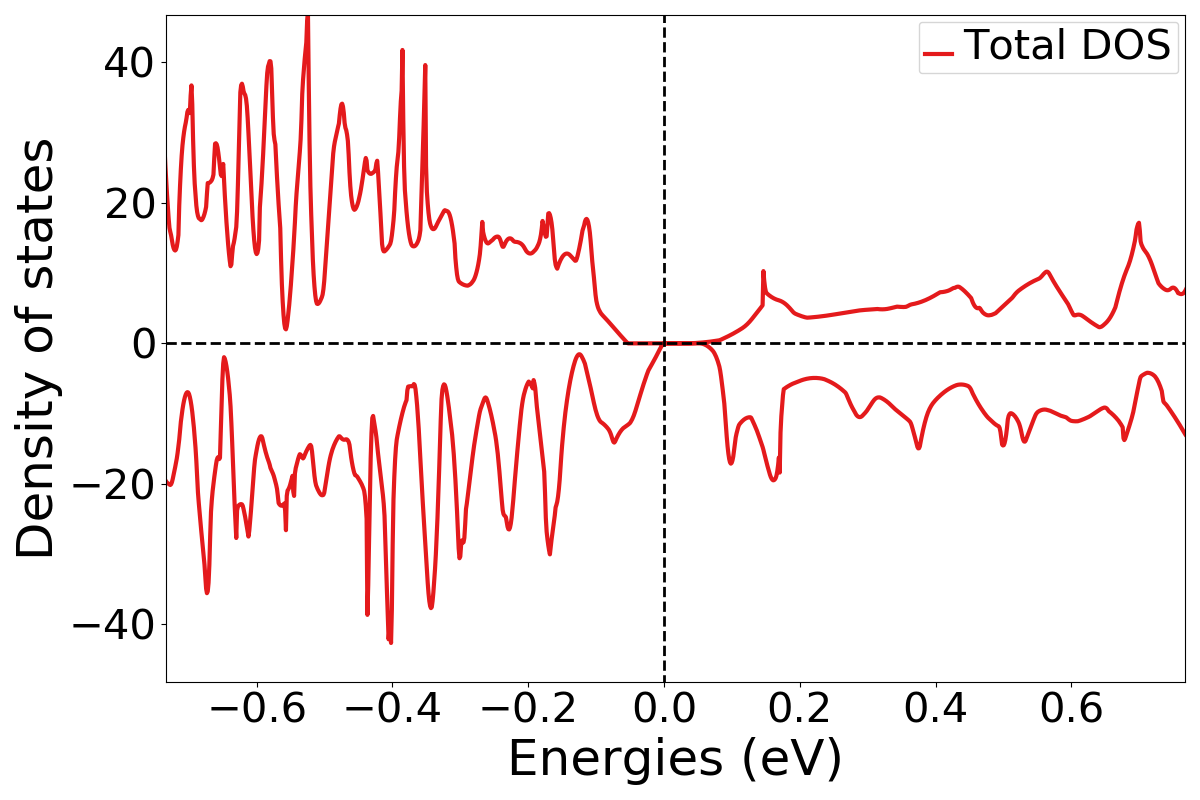
\includegraphics[width=\textwidth]{results/fesi2/DOS_A_toten.png}
	\end{subfigure}

	\begin{subfigure}{0.9\textwidth}
		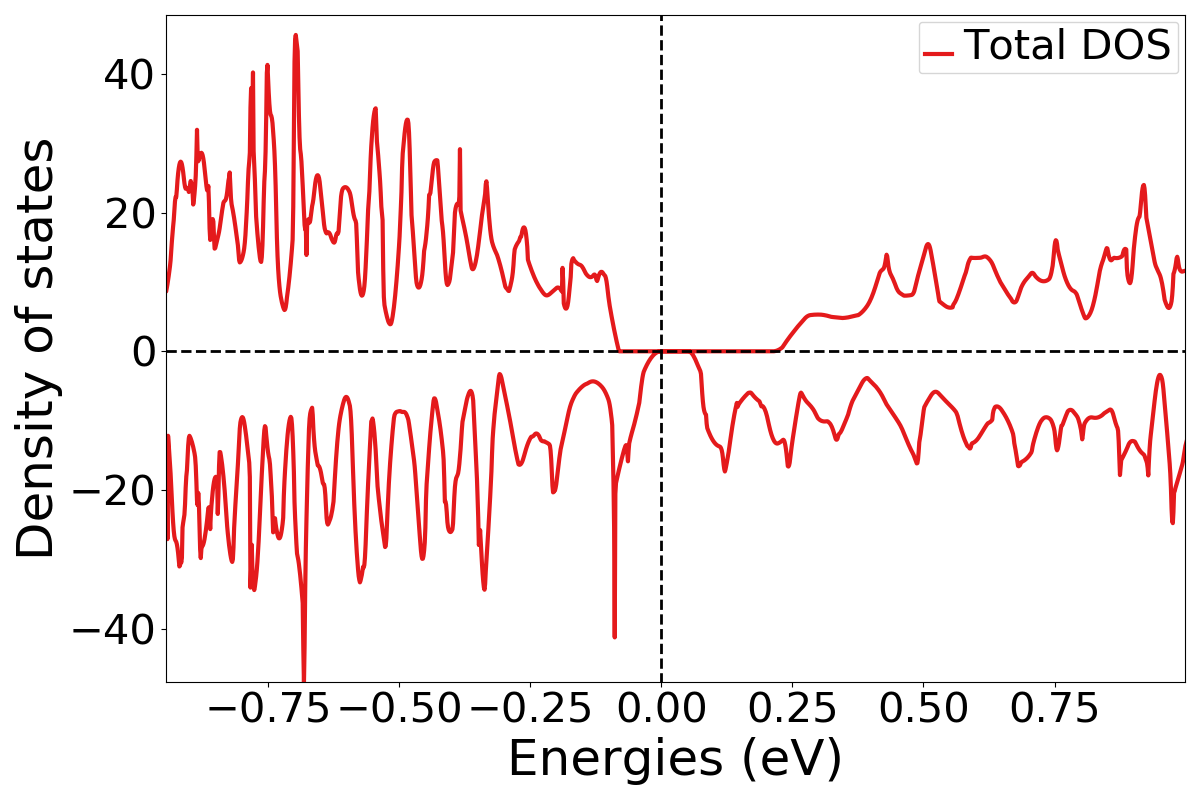
\includegraphics[width=\textwidth]{results/fesi2/DOS_B_toten.png}
	\end{subfigure}
	\begin{subfigure}{0.9\textwidth}
		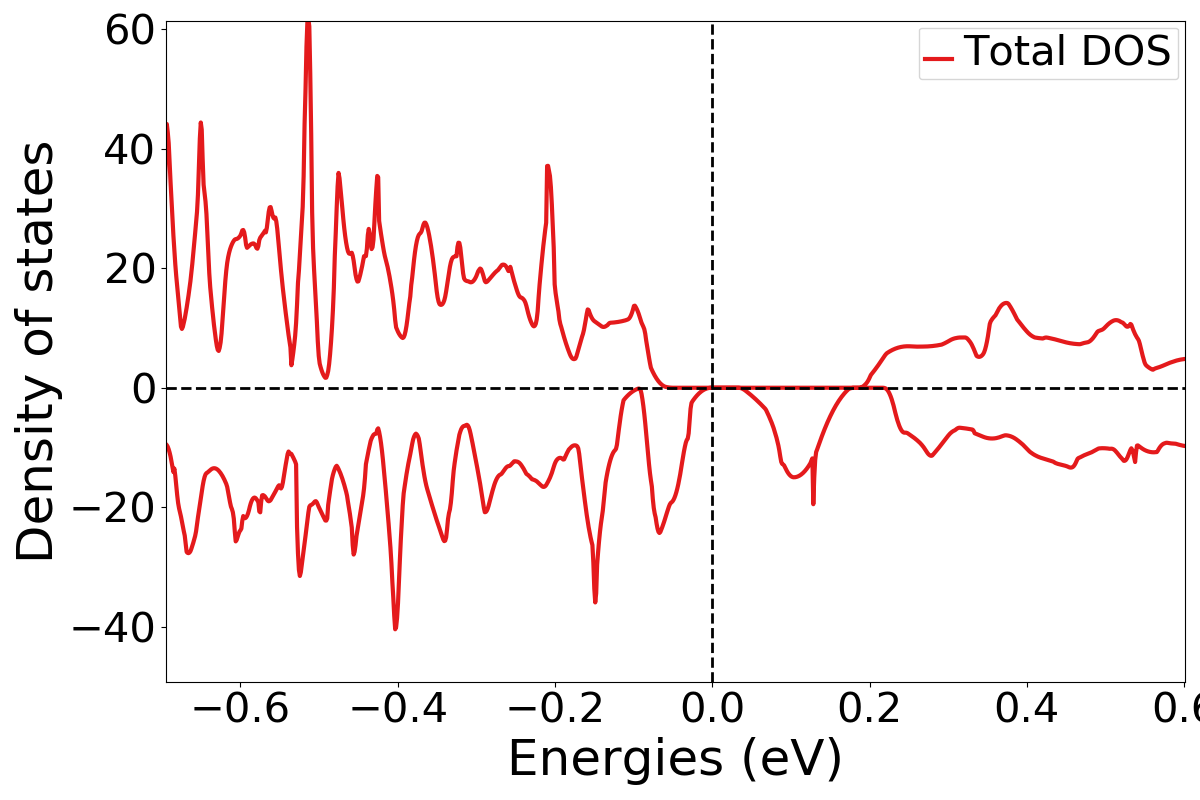
\includegraphics[width=\textwidth]{results/fesi2/DOS_C_toten.png}
	\end{subfigure}
\end{figure}
\begin{figure}[H]
	\centering
	\begin{subfigure}{0.9\textwidth}
		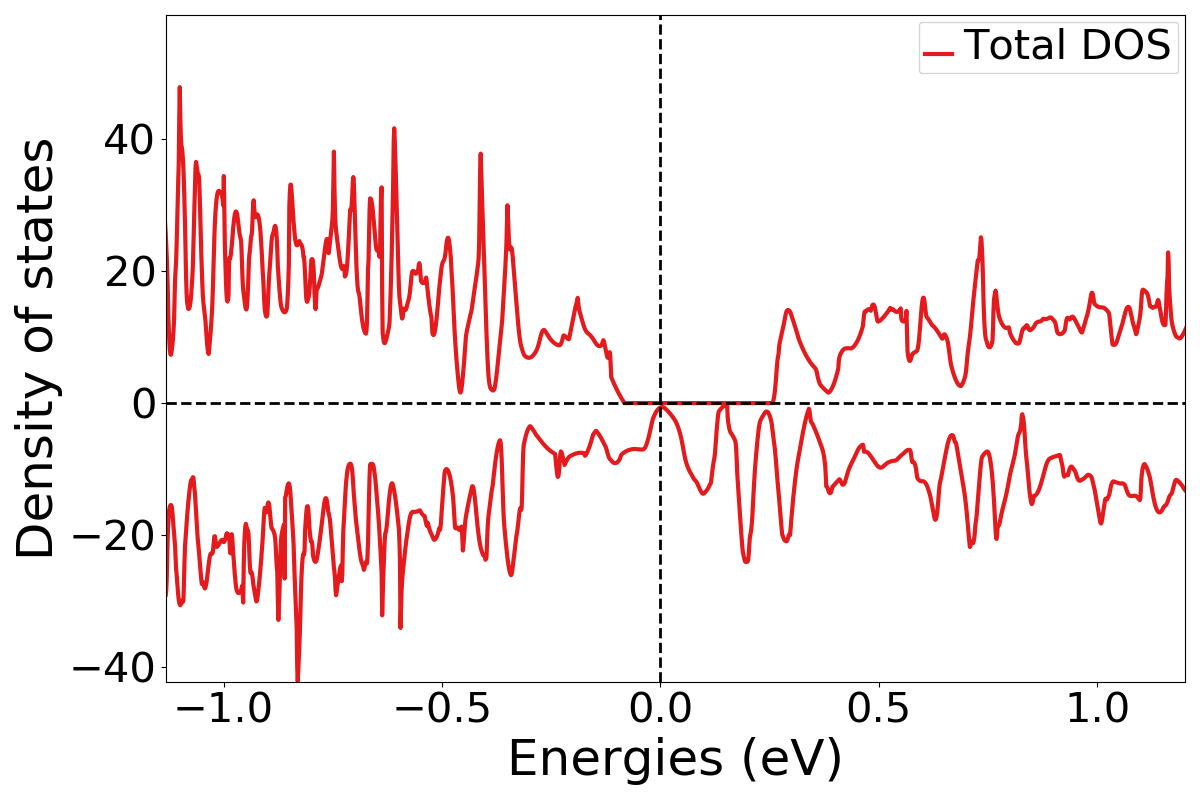
\includegraphics[width=\textwidth]{results/fesi2/DOS_D_toten.png}
	\end{subfigure}
	\begin{subfigure}{0.9\textwidth}
		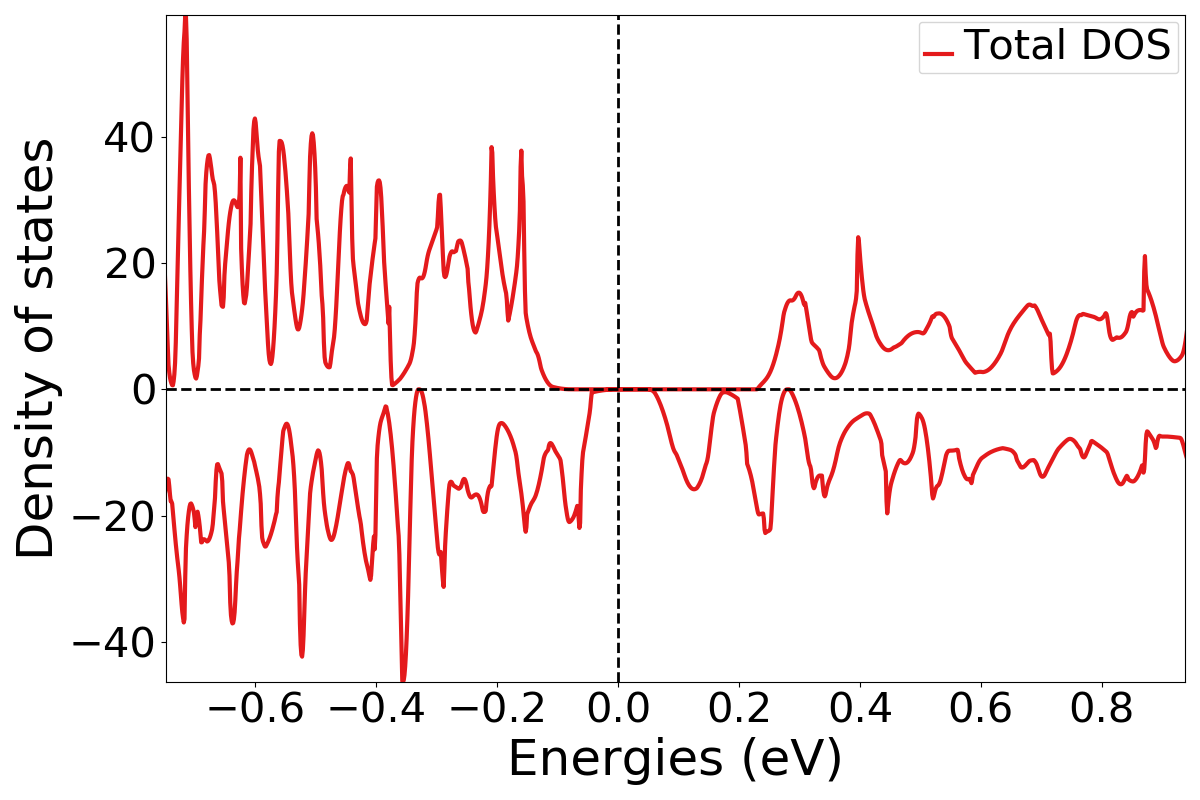
\includegraphics[width=\textwidth]{results/fesi2/DOS_E_toten.png}
	\end{subfigure}
	\caption{Density of states for structure A, B, C, D, E of $CFMNSi_2 (FeSi_2)$ SQSs (PBE GGA)}
	\label{dos_fesi2_gga}
\end{figure}

In spin polarized materials such as this one, the band gap can be extracted from the total DOS by the minimal width of unoccupied states around the Fermi energy. From figure .. we can observe two properties of the band gap. One, there is clearly a band gap in structures A, B, C, and E, and secondly, the band gap is significantly greater in the spin $\uparrow$ channel than spin $\downarrow$. This is especially evident for structure D, where we learn that the structure is metallic in spin down, but contain a sizable  gap in spin up.

The density of states, all though useful provide limited information.  For instance, the DOS in structure D point to a difference in spin states, but does not give any indication as to to why. Additionally, the density of states can be unreliable and prone to errors. As mentioned in section .., the smearing is important for accurate DOS calculations, preferably the tetrahedron smearing with Bloch correlations (TBS). In this project we experiences a significant difference between calculations with gaussian and TBS smearing in relation to the written band gap and the density of states band gap (More on this later). Moreover the DOS is very sensitive to computational factors such as number of points used in the DOS (NEDOS in VASP) and k-points (to solve the DOS integral, see section ..). For example, the band gap in structure C could only be seen in the density of states when increasing the number of points in the DOS from 2401 to 20000 points (this was not the case for the other structures). 

\begin{table}[H]
\centering
\begin{tabular}{@{}cccc@{}}
\toprule
Structure  & Spin-up & Spin-down & Total  \\ \midrule
\textbf{A} & 0.0814  & 0.0522    & 0.0281 \\
\textbf{B} & 0.2932  & 0.0523    & 0.0523 \\
\textbf{C} & 0.2355  & 0.0343    & 0.0343 \\
\textbf{D} & 0.3386  & 0         & 0      \\
\textbf{E} & 0.3078  & 0.0495    & 0.0495 \\ \bottomrule
\end{tabular}
\caption{Band gap (eV) with PBE in spin up and spin down channels of CFMN (fesi2) SQSs}
\end{table}

A more rigid method for both determining and investigating the energy bands is to study the Kohn-Sham eigenvalues. The eigenvalues are given for all energy bands for the given number of k-points used in the calculation, with listed energies and corresponding occupancy in both channels.  In table (..) above, we provide the relationship between the spin up and down channels in regards to the band gap, as read from the eigenvalues. In addition to validate and quantify the point expressed above about the gap in both spin channels, we can from the eigenvalues qualitatively differentiate structure D from the rest. From observing that for certain k-points, the occupancy does not transition from 1 to 0 directly between two bands, but rather contain one or more partially occupied bands in between, however only in the spin down channel. If we were to neglect this partially occupied states, and only consider bands with above 0.99 or bellow 0.01 occupancy, the band gap of structure D remain consistent in spin up, but we now observe a band gap in spin down around 0.05 eV and similarly thus for the total band gap of the structure. Again, this would have been extremely insightful to investigate with help of a band structure diagram.

\textbf{Something on the flaws of EIGENVALUES, bloch corrections yield un-physical eigenvalues in structures without band gap. Some times we find band gap from eigenvalues but not DOS or other script. What does the distance in bands between 1 occ and 0 occ mean?} 


As expressed previously, in this work we include 3 level of depths GGA (PBE), meta-GGA (SCAN) and hybrid functionals (HSE06). In table .. bellow we show the results from these functionals. 

\begin{table}[H]
\centering
\begin{tabular}{@{}cccc@{}}
\toprule
Structure  & PBE    & SCAN   & HSE06  \\ \midrule
\textbf{A} & 0.0281 & 0.0000 & 0.0207 \\
\textbf{B} & 0.0523 & 0.0890 & 0.1808 \\
\textbf{C} & 0.0344 & 0.0690 & 0.0196 \\
\textbf{D} & 0.0000 & 0.0000 & 0.0000 \\
\textbf{E} & 0.0495 & 0.1048 & 0.0133 \\ \bottomrule
\end{tabular}
\caption{Band gap of $CFMN (FeSi_2)$ SQSs with GGA (PBE), meta-GGA (SCAN) and hybrid-functionals (HSE06).}
\end{table}

The first fact we make notice of is that aside from A, all 3 methods agree on the presence of a band gap, but the actual value is under debate. We see a general trend that the SCAN functional find the largest gaps and HSE06 the lowest. This is an unexpected result, the general consensus is that hybrid functionals will extend on the band gap found by LDA or GGA functionals \textbf{Find reference!}. However we find one exception to this trend, in structure B the band gap increase from 0.05 to 0.09 and 0.18 eV. The most likely reason for this abnormal large gap is a consequence of the small number of k-points we had to employ in order for the calculations to converge. Recalling that the transition in in the PBE calculation was (0.250,0.000,0.250)-(0.000,0.000,0.000), comparing to HSE, the gap transition is between (0.500,0.000,0.000)-(0.000,0.000,0.000). Moreover, the point (0.250, 0.000, 0.250) in k-space is not included in the hybrid functional due to the narrow mesh (from IBZKIT file). Thus we may conclude that the large gap from HSE06 is a result of that the minimal gap is not encapsulated by the k-mesh. On the other hand, with the SCAN functional we also observe an increased band gap, and also a different band transition from (0.250,0.000,0.250)-(0.000,0.333,0.000) despite identical k-points used in PBE and SCAN. We find the same results in the other SQSs as well, ie that the band transition varies between the 3 functionals of the same SQSs. 

The most relevant result regarding the SCAN functional is that of structure A, in which both PBE and HSE06 finds a semiconductor, but SCAN does not. Similar to structure D, this is because the eigenvalues contain so-called defect states and non-physical occupancy. Neglecting these, we find a band gap of about 0.03 eV, which is in good agreement with the PBE value.     

With the HSE06 functional we find a band gap of 0.021 eV, with a transition (0.000, 0.500, 0.500) - (0.500, 0.000, 0.000). From the eigenvalues we find that the gap is 0.7 eV in the spin up channel, compared to 0.02 eV in spin down and total \textbf{See DOSCAR maybe?}. As stated previously, to converge HSE06 calculations we had to first perform the calculation with Gaussian smearing, then reapply the charge density of that calculation to perform the calculation again with TBC smearing. Interestingly, the result of the first calculation (Gaussian) yielded a band gap of 0.15 eV, (0.78 up and 0.15 down). However the eigenvalues contain defect states and is not apparent from the density of states. Without defect states the band gap is increased further to 0.25 eV. By reducing the smearing width from 0.05 to 0.005 we find a gap of 0.1 eV (0.21 up and 0.1 down) without any defect states, and that is shown in the density of states. \textbf{Include figure?} 

In structure B, we have calculated the band gap with both gaussian and TBC smearing for PBE and HSE06. From PBE, both methods agree on a band gap around 0.05 eV, but the gaussian method yield eigenvalues with defect states, and a metallic density of states. Without defect states the band gap from gaussian PBE is found to 0.17 eV. In this supercell, the SCAN functional find a total band gap of 0.088 eV from 0.15 eV up and 0.088 eV down, the eigenvalues are pure and the gap is well represented in the density of states. The hybrid functional of this SQS is in pretty good agreement despite of smearing method. From gaussian smearing and smearing width we find a gap of 0.15 eV (with defect states, 0.28 eV without). From reducing the smearing width we find a gap of 0.18 eV identical to TBC, without defects in the eigenvalues and represented in the density of states. 

Structure C is similar to B with PBE, where the smearing method produce similar band gaps, but the gaussian contain defect states. Interesting of this structure is that the SCAN functional result in an opposite gap to the PBE functional. With PBE, the gap was largest in spin up and limited by the down states. From Scan, we observe that the gap is about 0.11 eV in down, and 0.07 eV in up. HSE06 agree with PBE, and find that the spin up channel have a band gap of 0.17 eV and 0.032 eV in spin down. With gaussian smearing, we find HSE06 to yield a gap around 0.1 eV in both channels and 0.065 eV in total (with defect states).

In structure D, we observe the same result. From PBE, the we find a band gap in spin up around 0.33 eV, but a metal in spin down. If we remove the defect states, the spin up gap remain constant, but we now find small gap of around 0.05 eV in down and correspondingly in total. And from the SCAN functional, the inverse is true. ie we initially find a band gap for spin down electrons, but not spin up. The results of HSE06 for this supercell is similar to structure C, in agreement with PBE and disagreement with SCAN. The band gap from HSE06 is calculated to about 0.37 eV in up and 0 in down from gasuusan smearing. We find a total gap of 0.26 eV when overlooking the defect states in the eigenvalues. \textbf{Wait for ismear-5 HSE06 to finish}. 

Finally, we observe the same pattern again for structure E. The PBE functional find a large gap in up and near 0 in down with TBC smearing. And the gaussian smearing find a similar gap in spin up, and the small gap in spin down is consistent, but caused by defects. Removing these defects we find a gap in down around 0.16 ev resulting in an increased total gap. Also in this case, the SCAN functional finds a different band transition than PBE, despite identical k points and parameters. The gap is calculated to 0.15 eV in spin up, 0.11 eV in down and 0.10 in eV in total. The HSE06 calculations of this structure resemble that of structure A. With TBC, the band gap is very large in spin up, about 0.55 eV, but close to 0 in down. The gaussian smearing finds similarly a large gap in up (0.66 eV) and a larger spin down gap around 0.15 eV, with defect states and 0.16 eV without. This gap is not apparent in the density of states, but we have found merit that the gap could become viable, by reducing the smearing width, as in structure A.  

A concluding remark, why does only str B agree between gaussian and TBC in HSE06. And which method is more reliable, surely one would expect the gaps from HSE06 to be bigger than PBE/SCAN. But the tetrhaedon method is considered the most accurate? \textbf{This is discussion material!, rewrite this section, and try to make the summary more concise and less repeative, while still containing the same information}

At the risk of becoming repetitive and tedious, we still include this section where we walk though every SQS and the 3 functionals to make the reader aware of the differences and and disagreement we have observed in this study, both in relation to 5 SQSs of the same compound, but also from three highly praised exchange-correlation functionals.  
In conclusion, its very strange that the two smearing methods produce the same band gap in several instances, but that one of the channels is caused by defects in gaussian, but TBC find the same gap but without defects. And in addition, the large differences observed for HSE06 between the two methods is interesting. \textbf{I think I will include something like this in the summary/conclusion: Due to the disagreement between methods, SQS'sizes and etc, we may not confidently report a precise value of the band gap, but we can with some confidence conclude that we have found semiconducting high-entropy silicides.}   


To further compare and anlyze the 5 SQSs of CFMN (fesi2) high-entropy silicide, we investigate the local density of states (LDOS), given in figure \textbf{insert ref.} \textbf{These figures needs work for how they are presented, include all? Or just 1?, full view or zoomed around EF, fix axes ticks font size and weight and figure size. Redo structre C with the DOS from NEDOS}

\begin{figure}[H]
\centering
	\begin{subfigure}{\textwidth}
		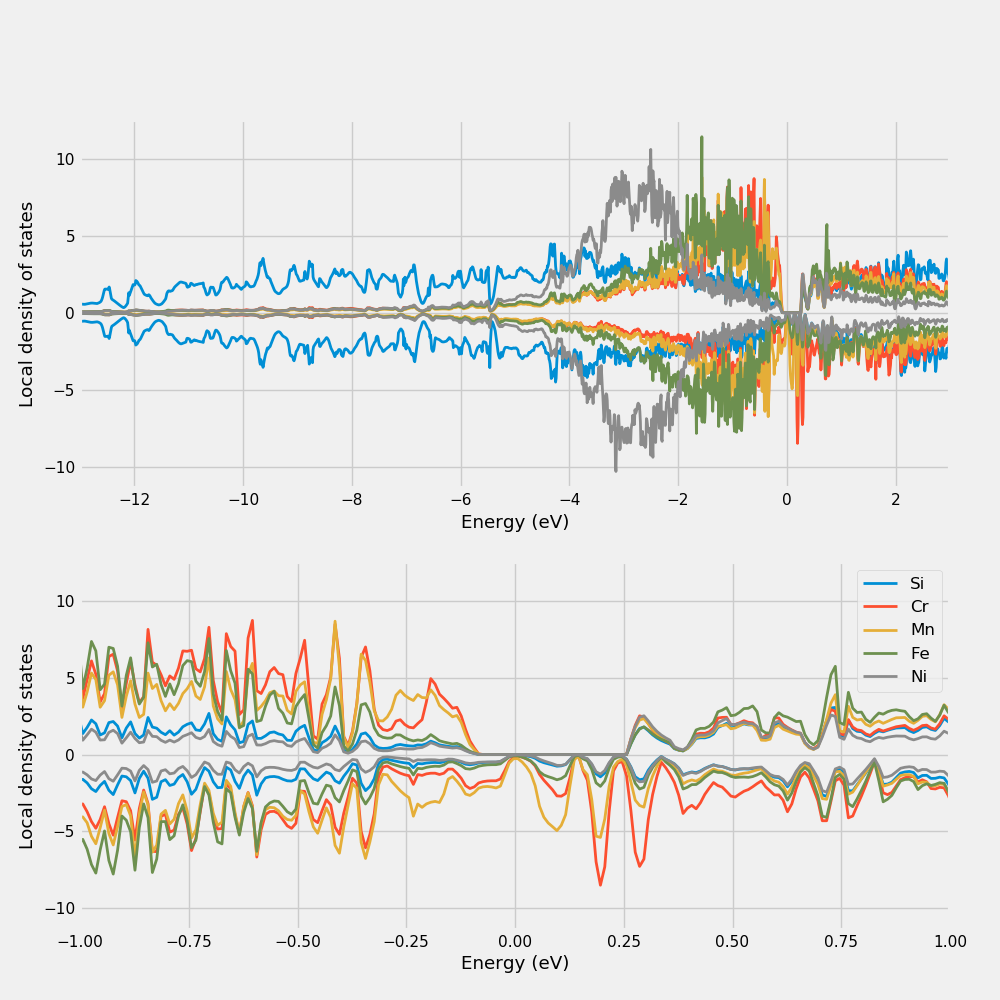
\includegraphics[width=\textwidth]{results/fesi2/A_LDOS.png}
		\caption{A}
	\end{subfigure}
	\begin{subfigure}{\textwidth}
		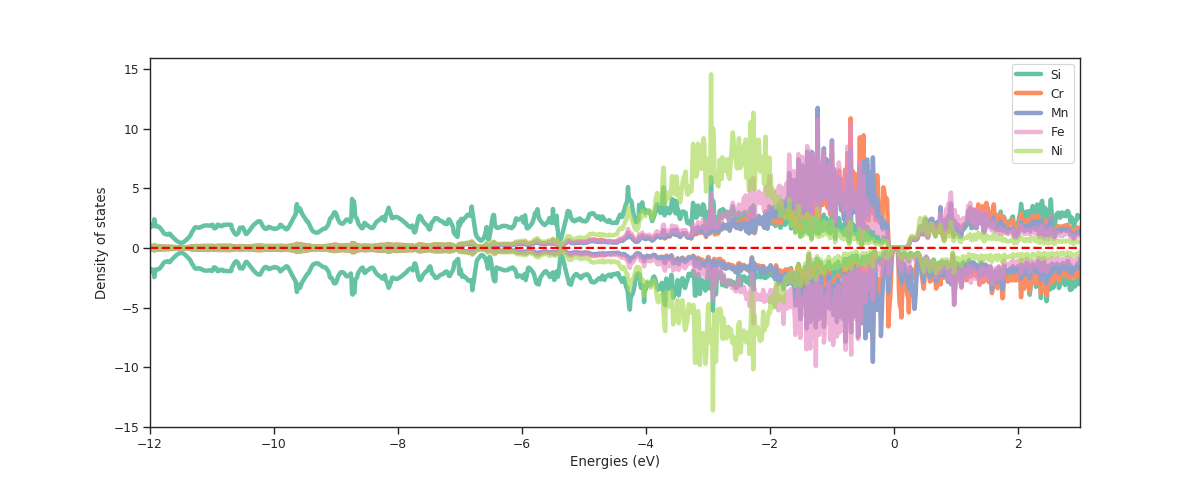
\includegraphics[width=\textwidth]{results/fesi2/B_LDOS.png}
		\caption{B}
	\end{subfigure}
	\begin{subfigure}{\textwidth}
		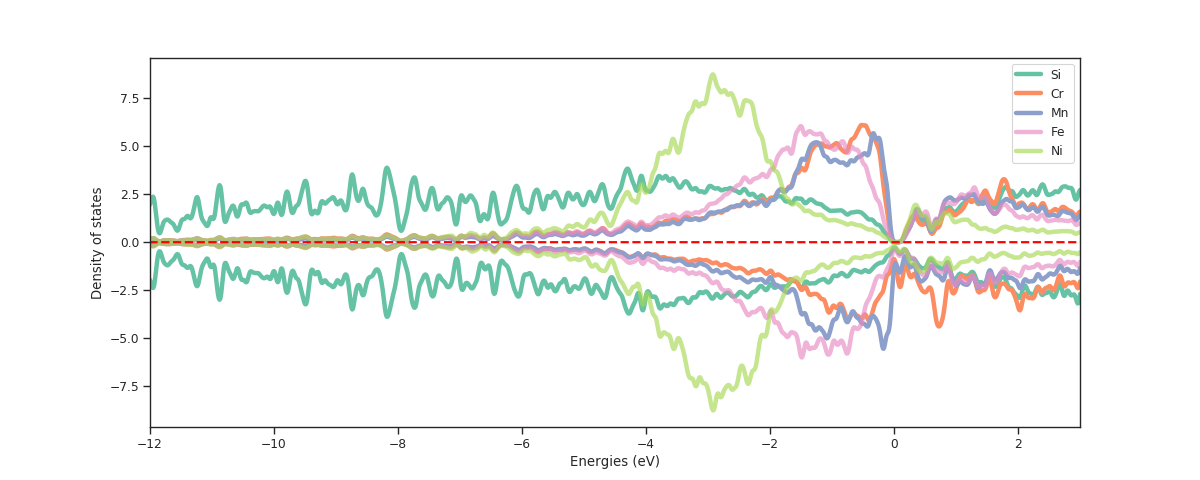
\includegraphics[width=\textwidth]{results/fesi2/C_LDOS.png}
		\caption{C}
	\end{subfigure}
	\begin{subfigure}{\textwidth}
		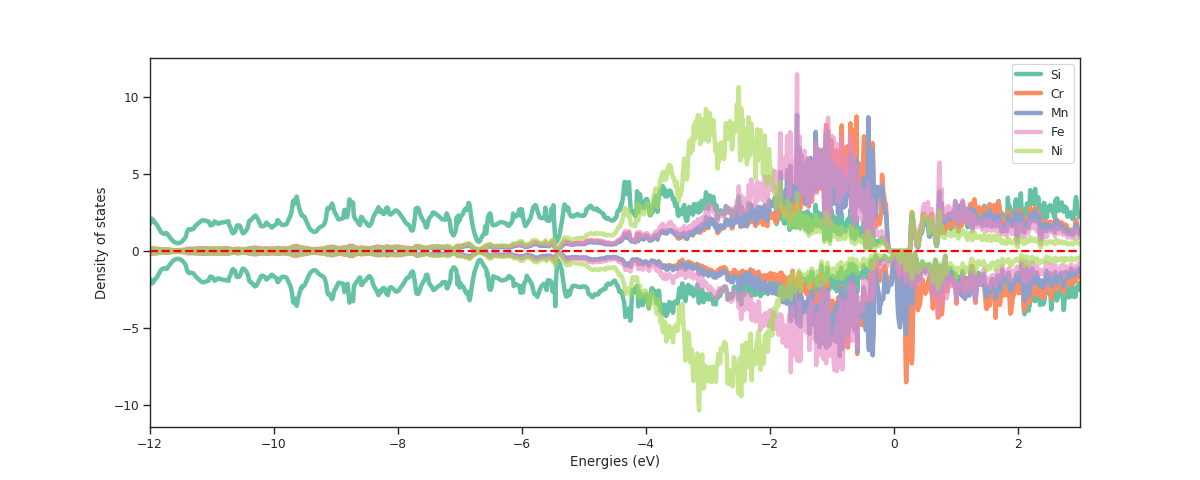
\includegraphics[width=\textwidth]{results/fesi2/D_LDOS.png}
		\caption{D}
	\end{subfigure}
\end{figure}		
\begin{figure}[H]
	\centering	
	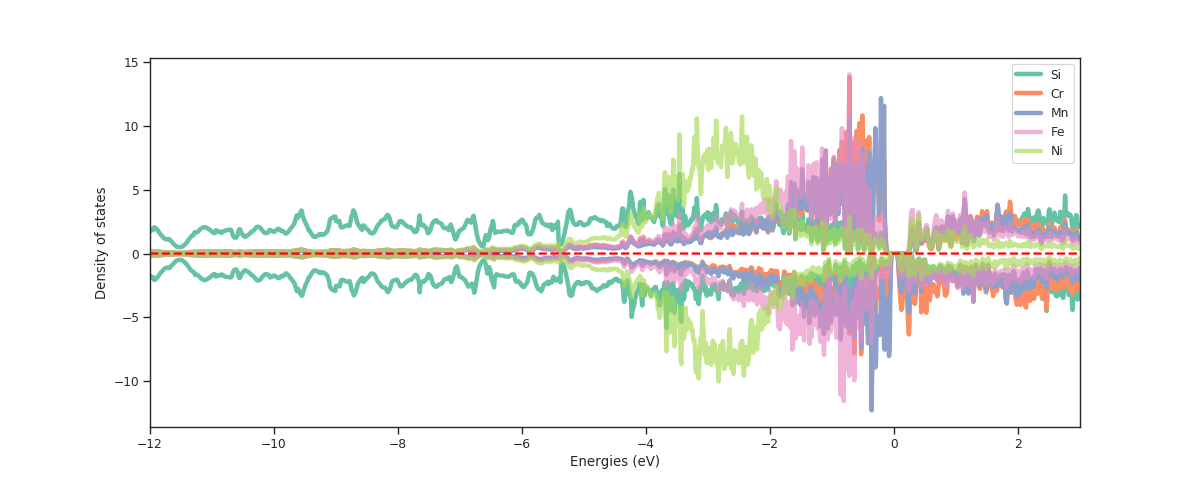
\includegraphics[width=\textwidth]{results/fesi2/E_LDOS.png}
	\caption{E}
\end{figure}

From these figures, we observe a typical pattern throughout the 5 SQSs, in which energies much lower than $E_F$ is dominated by s electrons corresponding to silicon atoms. At slightly higher energies, we see strong hybridization of Si p electrons and 3d electrons of TMs. We observe for both spin channels that Ni lie at the lowest energies of the 3d elements, followed by iron and then manganese and chromium very close to the fermi energi. Above the fermi enery, we obsere a more equal contribution from all elements, however energies slgihtly above EF is slightly favored by Fe in spin up states, and Cr in spin down. For higher energies, the highest LDOS is attributed to Si and Cr, while elements such as Ni, Fe and Mn have  a lesser role on the total DOS. One key distinction of str D is a heavy amount of Manganese at energies right above Ef in spin down, in contrast to the other structures that are dominated by Cr at this energy. An additional distinction between the five SQSs is the intensity of the local density of states, in the structures with the highest band gap, structures B and E, the local density of states is slightly higher. In particular, structure E show high LDOS of Cr and Mn close to Ef in spin up, and Ni in structure B at slightly lower energies.  

If we now consider the probability distribution functions (PDFs), shown in figure \textbf{insert ref!}. From these figures there is a lot of useful information to investigate. With the aid of the ICSD (insert citation), we can locate the expected PDFs based on recent research and experiments from a host of different compounds. As our compound contain a total of 15 different bonds, comparing each one of these for all 5 supercells to the ICSD values would be an exhaustive process. For our purpose we are satisfied by comparing the 4 different metal-Si bonds and note ourselves of key distinctions. We find that the preferred bond-length of TM-Si is observed at two values, the most dominant being the shorter of the 2. For Fe-Si these are between 2.25-2.75 and 4-5, Mn-Si 2.25-2.75 and 3.5-5. Ni-Si lie between 2.25-2.5 and 3.85-5 and Cr-Si between 2.35-2.65 and 4-5. 

\textbf{These figures need work, maybe not include all or? I notice that the same color is used twice several places, also some lines are covered by other. To actually read info from these I had to study them in matplotlib and zoom in and out}
\begin{figure}[H]
\centering
	\begin{subfigure}{\textwidth}
		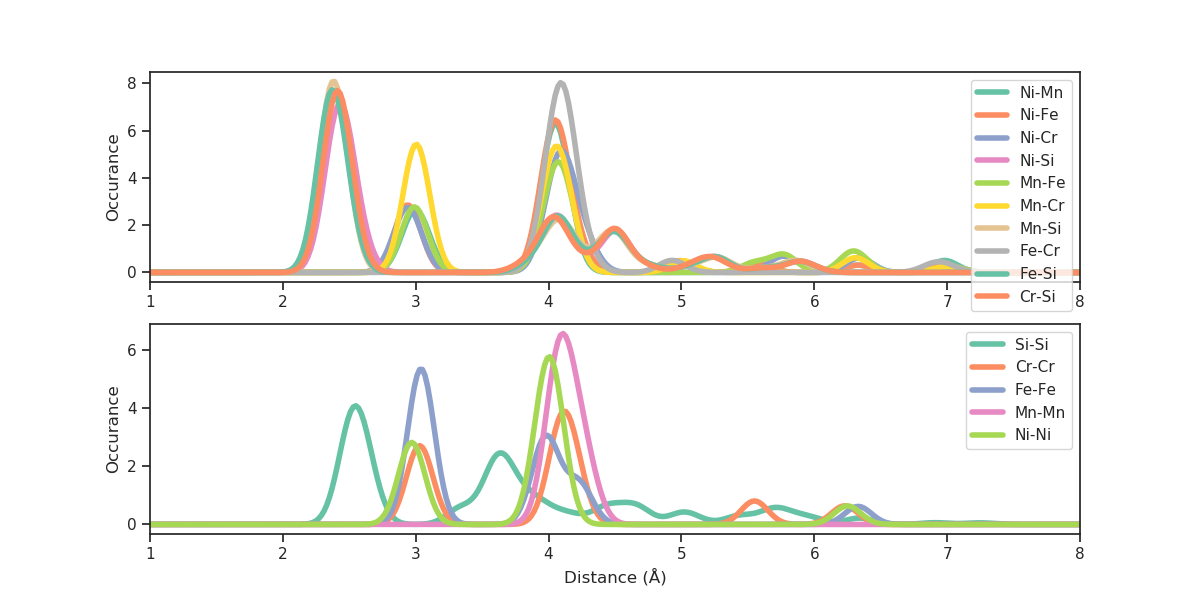
\includegraphics[width=\textwidth]{results/fesi2/A_PDF.png}
		\subcaption{A}
	\end{subfigure}	
	\begin{subfigure}{\textwidth}
		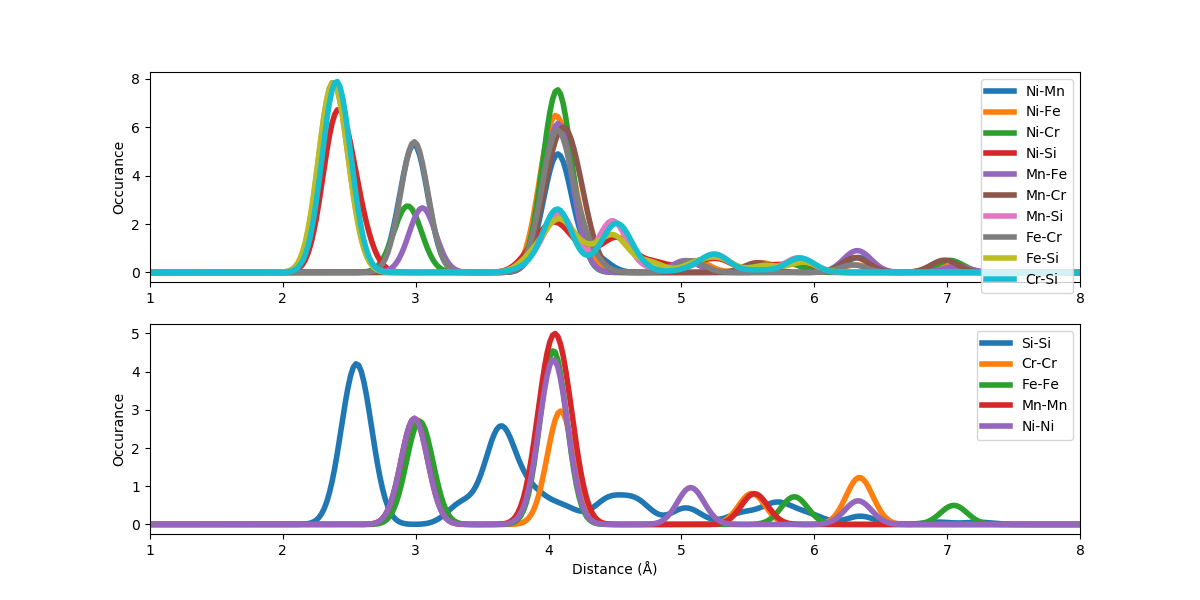
\includegraphics[width=\textwidth]{results/fesi2/B_PDF.png}
		\subcaption{B}
	\end{subfigure}
	\begin{subfigure}{\textwidth}
		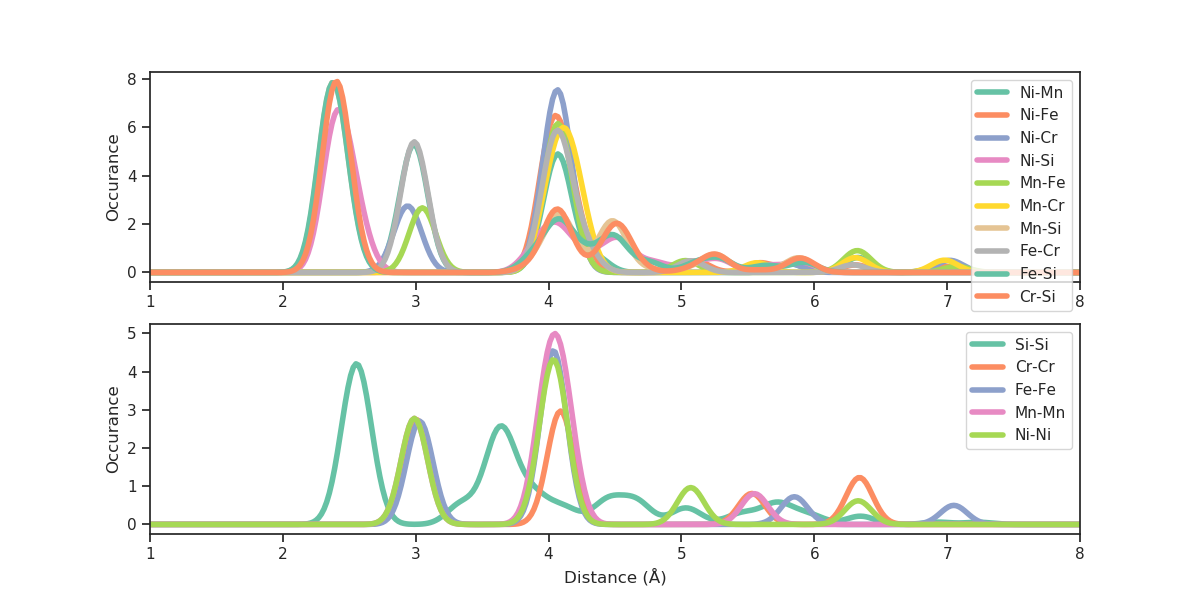
\includegraphics[width=\textwidth]{results/fesi2/C_PDF.png}
		\subcaption{C}
	\end{subfigure}
\end{figure}
\begin{figure}[H]
\centering
	\begin{subfigure}{\textwidth}
		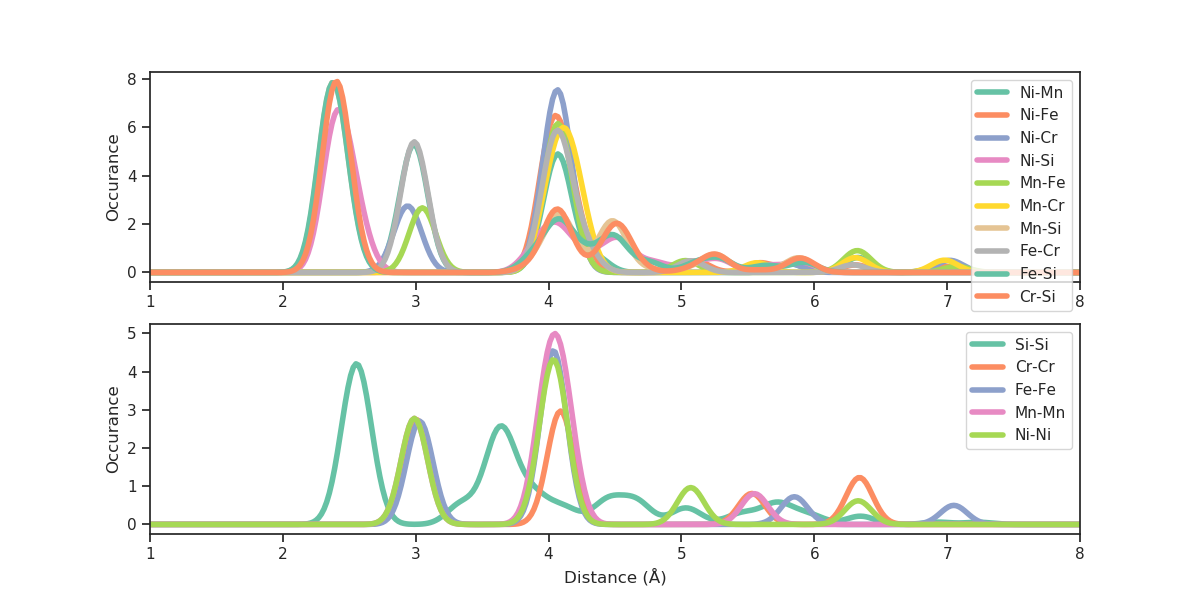
\includegraphics[width=\textwidth]{results/fesi2/D_PDF.png}
		\subcaption{D}
	\end{subfigure}
	\begin{subfigure}{\textwidth}
		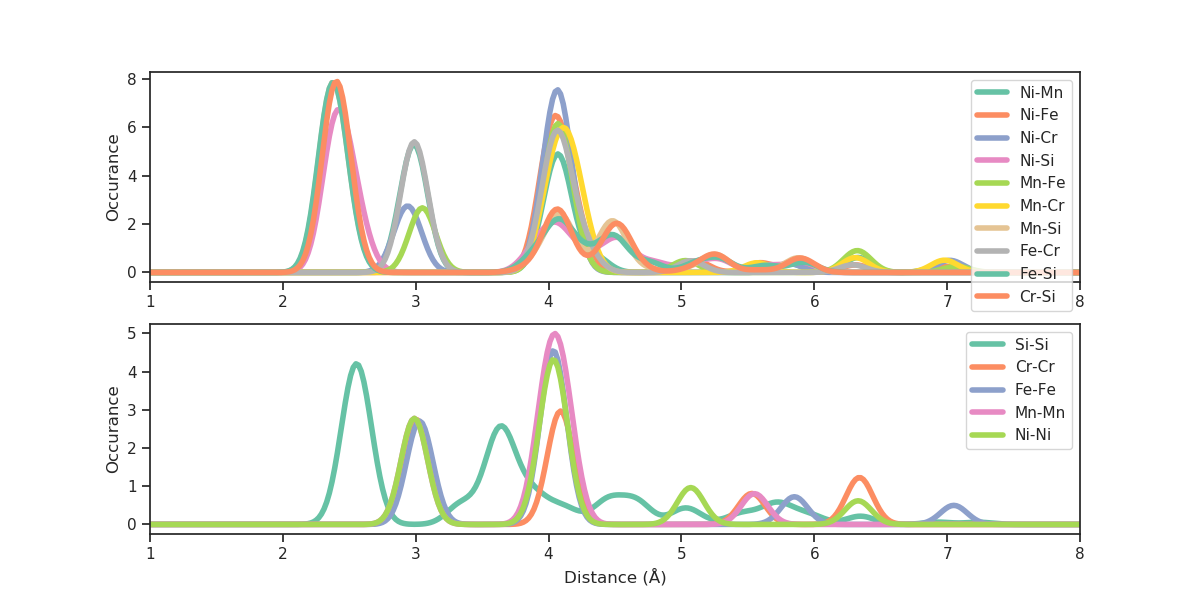
\includegraphics[width=\textwidth]{results/fesi2/E_PDF.png}
		\subcaption{E}
	\end{subfigure}
\end{figure}

\textbf{Finish discussion pdfs, introduce CHGCAR}

\begin{figure}
	\begin{subfigure}{\textwidth}
		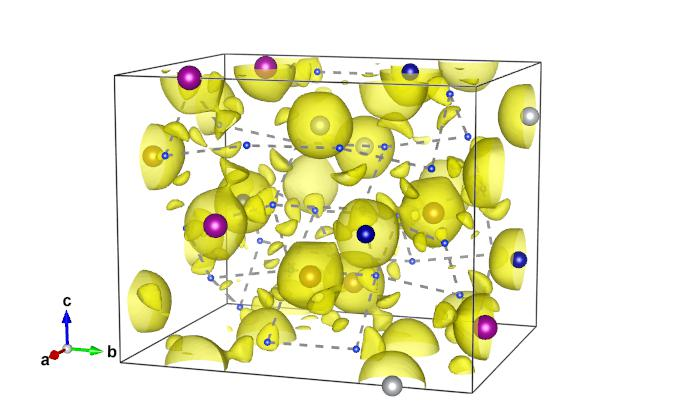
\includegraphics[width=\textwidth]{results/fesi2/B_CHGCAR.jpg}
		\caption{Structure B}
	\end{subfigure}
	\hfill
	\begin{subfigure}{\textwidth}
		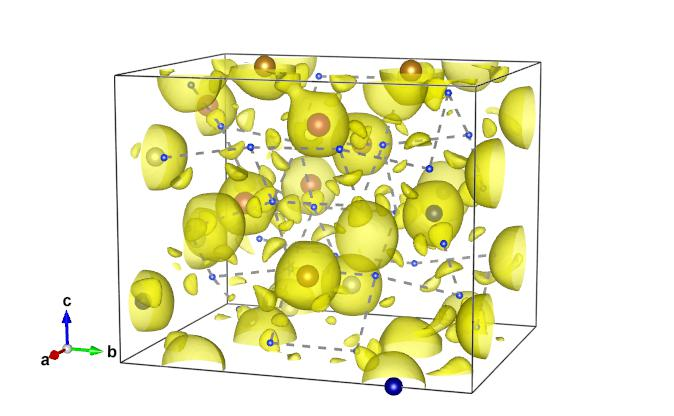
\includegraphics[width=\textwidth]{results/fesi2/D_CHGCAR.jpg}
		\caption{Structure D}
	\end{subfigure}
\end{figure}

At the surface, figure .. show that are supercells are in good agreement with the listed values for Tm-Si bonds, with the most occurring bond length falling at around 2.4 Å for all TMs, and some bonds at around 4.1 Å. The relative height of the peaks follow a similar trend, Fe-Si, Mn-Si, and Cr-Si all lie close to 8 for the first peak at 2.4 Å, and Ni-Si slightly bellow around 7. \textbf{More on the PDFs?}


Lastly we include the charge density of blabla, \textbf{something on these.}

\subsection{Permutations of CFMN (fesi2)}


\subsection{Other composistions (fesi2)}

\section{two iron, one silicon}

\begin{table}[H]
\centering
\begin{tabular}{@{}cccc@{}}
\toprule
Structure  & Total energy/atom (eV) & Final magnetic moment (?) & Band gap (eV) \\ \midrule
\textbf{A} & −7.2129                & 19.3167                    & 0.0000        \\
\textbf{B} & −7.2110                & 21.0030                    & 0.0000        \\
\textbf{C} & −7.2042                & 19.0002                    & 0.0000        \\
\textbf{E} & −7,2077                & 17.4200                    & 0.0000             \\
\textbf{Mean} & −7.2090            & 19.1850                  	 & -        \\ 
\textbf{Std} & 0.0038				  & 	1.4688						& -				\\ \bottomrule
\end{tabular}
\caption{Total energy per atom, final magnetic moment, and band gap (PBE) of $(CrFeCoNi)_2Si$  }
\label{table:fesi2_summary}
\end{table}  

\section{CFMN in the $CrSi_2$ and $MnSi_{1.75}$ ($Mn_4Si_7$) unit cell}

\section{Overview}


\textbf{I think its relevant and interesting to in-depth analyze structure B, D, and E. B because of large band gap. D because no band gap, and E because this well represents the other structures A and C. }
One difference is the KS eigenvalues. Str D have both partial occupancy and nonphysical occupancy, ie above 1 and bellow zero both in PBE and HSE06. This is not the case for structures that exhibited band gaps. Here we have clear transition from 1 to 0. Without having done a broad investigation of all material. This seems to be the case in other compositions and cells and permutations as well. Where both partial occupants and nonphysical occupations result in metallic structures. Calculating the band gap with strict 1 and 0 conditions, lead to small band gaps in most structures. Furthermore, in structures of Fe2Si, the difference in band where occupation transition from 1 to 0 between up and down, increases hugely compared to FeSi2 structures, talking close to 20 bands, opposed to maybe 2-5. 
